\subsection{Meshes in finite element algorithms}

Meshes are fundamental tools in Finite Element algorithms. Polygonal meshes are particularly useful for their flexibility in representing complex geometries. This section describes a mesh-building strategy using polygonal meshes over polygonal domains.

\subsection{Building a mesh}

\begin{figure}[!ht]
    \centering
    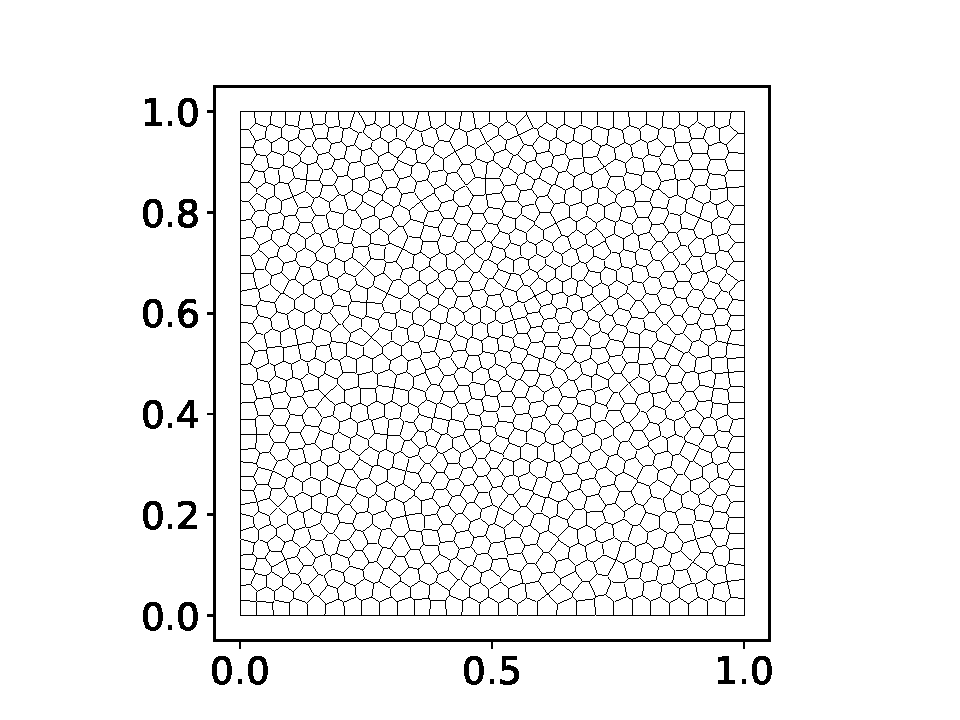
\includegraphics[trim=2cm 0.5cm 2cm 0.5cm, clip, width=0.45\textwidth]{meshes/uniform/square_1000.pdf}
    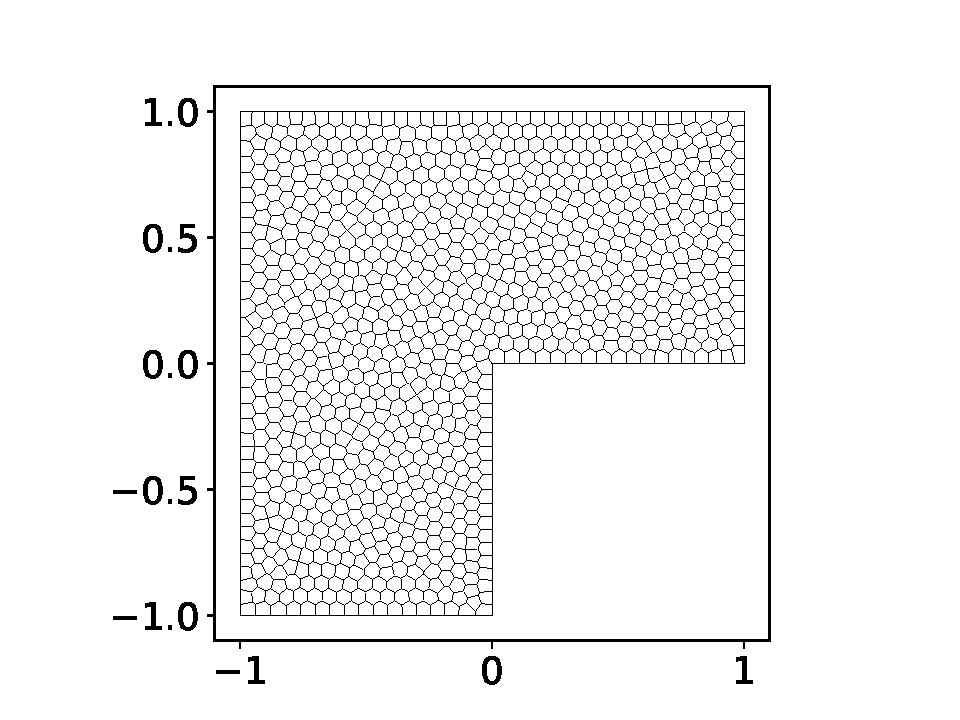
\includegraphics[trim=2cm 0.5cm 2cm 0.5cm, clip, width=0.45\textwidth]{meshes/uniform/lshape_1000.pdf}
    \caption{Square and L-shaped meshes over polygonal domains with $N = 1000$ elements. These examples illustrate the mesh quality and structure.}
\end{figure}

The mesh-building strategy, adapted from \cite{Talischi2012}, involves the following steps:

\begin{enumerate}
    \item Generate a Voronoi diagram to partition the domain into regions based on point locations. This step divides the domain into regions, each associated with one of the points, thereby laying the foundation for the mesh structure.
    \item Refine the mesh by adjusting point positions to minimize element distortion. Lloyd's algorithm iteratively relocates points to achieve a more regular mesh, reducing irregularities and improving mesh quality.
    \item Remove or adjust very small edges to enhance mesh quality and stability. This step addresses elements that are too small, which could negatively impact the mesh's performance and accuracy.
    \item Analyze the connectivity and arrangement of mesh elements to ensure proper structure. This evaluation ensures that the mesh elements are appropriately connected and organized.
    \item Calculate properties such as element areas and the largest simplices\footnote{Necessary for the evaluation of the penalization coefficients.}.
\end{enumerate}

The \lstinline{mesh_diagram} function plays a crucial role in this process. It requires:

\begin{enumerate}
    \item A polygon defining the mesh's domain. This polygon represents the boundary within which the mesh will be generated.
    \item A number of points specifying the density of the mesh. The quantity of points determines how densely the mesh is populated within the domain.
    \item A reflection flag for accommodating non-convex\footnote{\lstinline{mesh_diagram} may fail to produce a mesh for a non-convex domain, despite the checks that are performed.} polygons by reflecting points relative to the boundary and vertices. This flag is used to adjust the mesh generation process for complex polygon shapes.
\end{enumerate}

The function initializes each cell with the polygon (or bounding box for non-convex domains) and refines it using bisectors of all points. Lloyd's algorithm is used for relaxation to enhance mesh quality.

Post-processing involves collapsing small edges to maintain the overall shape and correcting reflection-induced errors. The final mesh is then evaluated by checking element areas and simplices to ensure desired properties.

\newpage
\subsection{A code snippet}

The following code snippet demonstrates the mesh-building process:

\lstinputlisting[style=cpp, firstline=11]{../snippets/square_mesh.cpp}

This snippet illustrates how to set up and execute the mesh-building procedure from the user's perspective, showing the key functions and their application in practice.